\documentclass[graphicx,amsmath,cite]{jarticle}

% レイアウトパラメータ
\renewcommand{\topfraction}{0.9}
\renewcommand{\bottomfraction}{0.9}
\renewcommand{\dbltopfraction}{0.9}
\renewcommand{\textfraction}{0.1}
\renewcommand{\floatpagefraction}{0.9}
\renewcommand{\dblfloatpagefraction}{0.9}

% 余白
\setlength{\headheight}{0mm}
\setlength{\headsep}{0mm}
\setlength{\topmargin}{-8.0mm}
\setlength{\oddsidemargin}{-10.4mm}
\setlength{\evensidemargin}{-4.4mm}
\setlength{\textwidth}{18cm}
\setlength{\textheight}{254.3mm}
\setlength{\columnsep}{10mm}

% 各グラフのサイズ
\def\system_eps_scale{0.87}
\def\muscle_eps_scale{0.38}
\def\graph_eps_scale{0.54}
\usepackage[dvipdfmx]{graphicx}
\usepackage{here}

%上からのフロート数の上限
%\setcounter{topnumber}{3}

\newcommand{\bm}[1]{\mbox{\boldmath $#1$}}

\makeatletter
\def\@cite#1#2{$^{\hbox{\scriptsize{#1\if@tempswa , #2\fi})}}$}
\def\thebibliography#1{\section*{参考文献\markboth {参 考 文 献}{参 考 文 献}}
\list {\arabic{enumi})}{\settowidth\labelwidth{[#1]}\leftmargin\labelwidth
\advance\leftmargin\labelsep\usecounter{enumi}}
\def\newblock{\hskip .11em plus .33em minus .07em}\sloppy
\sfcode`\.=1000\relax}
\long\def\@makecaption#1#2{\small \vskip 10pt \setbox\@tempboxa\hbox{#1 #2}
\ifdim \wd\@tempboxa >\hsize \unhbox\@tempboxa\par \else \hbox
to\hsize{\hfil\box\@tempboxa\hfil} \fi}
\def\fnum@figure{Fig. \thefigure}
\def\fnum@table{Table \thetable}

\def\section{\@startsection {section}{1}{\z@}{1.5ex plus .5ex minus .2ex}{1.8ex plus .2ex}{\large\center\bf\gt}}
\def\subsection{\@startsection {subsection}{1}{\z@}{1.5ex plus .5ex minus .2ex}{1.8ex plus .2ex}{\bf\gt}}
\def\subsubsection{\@startsection {subsubsection}{1}{\z@}{1.5ex plus .5ex minus .2ex}{1.8ex plus .2ex}{\bf\gt}}



\pagestyle{empty}
\makeatother
%--------------------------------------------------------------------------
\begin{document}

\twocolumn[
\begin{center}
{\Large\gt\bf CPGシナジー・筋シナジーに基づく歩行解析} 
\begin{tabbing}
\hspace{2mm}横浜国立大学\=\hspace{1mm}大学院\hspace{1mm}理工学府\hspace{1mm}数物・電子情報系理工学専攻\hspace{1mm}情報システム教育分野  \hspace{2mm}% \=
   
\\ 20NC417   \hspace{3mm}   松井 寿樹  \hspace{3mm}%\=
所属%\=
:島研究室 
\hspace{2mm}令和2年度 新入生課題 \hspace{3mm} \=2020年5月5日
    \
\end{tabbing}
\end{center}
]
\setlength{\baselineskip}{11pt} %行間の調節はここを変える
{\small
%\baselineskip 8mm %%%%%%%%%%%%%%% 行間変更
\section{はじめに}
\label{sec:intro}

平成30 年時点において日本の65 歳以上の高齢者人口が総人口にしめる割合は28.1\% となっており\cite{elderly},今後も高齢者の割合が増加していくことは言及するまでもない.高齢者の抱える大きな問題として加齢に伴う歩行能力の低下がある.歩行は日常生活において基本的な動作の1 つであり,歩行能力の低下は生活機能の低下へとつながる.加齢に伴う歩行能力の低下の要因として,筋力,バランス能力や神経系機能の低下があると指摘されている\cite{neural1}\cite{neural2}.筋力やバランス能力に関しては多くのトレーニング方法が提案されているのに対し,歩行に関わる神経系機能に関しては,いまだその詳細や評価法が不明である.歩行に関わる神経系機能の評価法が確立すれば,新たな歩行能力の改善に向けたトレーニングやリハビリテーション法の提案や効果検証などへ応用できる可能性がある.

歩行のような周期的な運動(以下,リズム運動と呼ぶ) はCentral Pattern Generator (CPG) と呼ばれるリズム生成器により実現しているとされ,これまでにヤツメウナギなどの生物の脊髄内に存在することが確認されている\cite{cpg}. また,人間にもCPG が存在すると考えられており,Dimitrijevie らは脊髄損傷患者の脊髄硬膜外に特定の電気刺激を与えることで麻痺している下肢部にリズム運動が誘発されることを報告している\cite{human}.これまでに,リズム運動をCPG に基づいてモデル化する試みが多くなされており,たとえばCPG モデルを使用して2足ロボットの歩行リズム生成の実現\cite{robot} やパーキンソン病患者の下肢リズム運動の表現および評価の試み\cite{perkinson} が行われてきた.このようにCPGモデルに基づいたリズム運動のシミュレーションやモデルパラメータを使用した運動評価が可能である.

しかしながら,人間の運動を表現することができるCPG モデルのモデル構造決定やモデルパラメータの決定方法が大きな課題である.これまでに,CPGのモデル構造として神経振動子を用いたMatsuokaモデル\cite{matsuoka} や蔵元モデル\cite{kuramoto} などが提案されており幼児の早期歩行をモデル化する試み\cite{infant} や補償歩行の解析\cite{impaired} などからもモデルの有用性が示されている.ただし,これらのCPG モデル単体では急激な運動リズムの変化や各周期ごとに周期や振幅が変化するような運動を表現するのは困難であった.これに対し,複数のCPGにより構成されるCPGのモデルとして,非線形振動子を用いた非定常なリズム運動を表現可能とするCPGシナジー仮説が考案され,モデルパラメータの比較からパーキンソン病患者の指タップ運動評価が試みられている\cite{shima}.また,考案されたCPGシナジーモデルに基づいた歩行解析・評価が行われ,結果からモデルパラメータによる非定常リズム運動の評価の可能性が示されている\cite{seo}.しかしながら,CPGシナジー仮設によって示された基本の運動リズムパターンを生成する複数のCPG が人間に存在しているかは明らかになっておらず,モデルベースでの歩行評価を実現するためには構成論的なアプローチや生物学的な観点からのより詳細な検討が必要である.

そこで本研究では,体重免荷装置を用いたより複雑な歩行状態の計測や,歩行時の計測データから抽出したCPGシナジー・筋シナジーに基づく歩行解析を行うことで,先行研究から発展したより詳細な検討を行う.

以下,2 章では先行研究について,3 章では研究方針について説明する.4 章では新入生課題の結果について,5 章で新入生課題に対するコメントを述べる.


%------------------------------------
\section{非線形振動子型CPGシナジーモデルに基づく歩行解析\cite{seo}}
\label{sec:mwl}
%------------------------------------

歩行に関わる神経系機能の評価法の確立を目指して,CPGの出力として非線形振動子モデル(Matsuokaモデル\cite{matsuoka})を採用したCPGシナジーモデル\cite{shima}に基づいた歩行評価・解析が行われている.図\ref{system}に歩行解析のシステム図を示す.歩行の計測には,モーションキャプチャ,左右ベルト分離型トレッドミル,PC を使用する.計測中のトレッドミルの速度をPC で制御し,トレッドミルからはベルトの速度データおよび,左右の床反力を取得する.左右のベルト速度を調整することで,通常歩行だけでなく変則的な歩行の再現が可能である.被験者には赤外線マーカを装着し,モーションキャプチャを用いて,トレッドミル上での歩行を計測する.得られた計測データから算出した身体関節角度(リズム信号) を用いてCPG シナジーモデルパラメータ・非線形振動子パラメータの抽出を行うとともに,得られたパラメータに基づき評価を行う.歩行計測・解析の手順は以下のとおりである.

\begin{enumerate}
  \item トレッドミル上で通常歩行と右側のベルト速度のみを半分に変更した変則歩行について,脚関節角度の計測を通常歩行→変則歩行→通常歩行の順に行い,リズム信号\bm{d}(t)とする.
  \item CPGシナジーモデルパラメータ(CPG パターン\bm{C},重み係数\bm{w},時間シフト\bm{t})をNMF(非負値行列因子分解)の乗法更新アルゴリズムを用いて,非線形振動子パラメータ($\bm{w}_{i,j} ,\bm{b}_{i},\bm{T}_{ri},\bm{T}_{ai}$)をGA(遺伝的アルゴリズム)を用いてリズム信号\bm{d}(t) から再帰的に算出する.
  \item 歩行状態の変化によって抽出されたパラメータがどのように変化するかを比較する.
\end{enumerate}

解析結果を図\ref{result}に示す.まず通常歩行から変則歩行に変化したとき,CPGパターンの変化,重み係数変動の増加,時間シフト値の増加が見られた.この結果から,モデルパラメータに運動の変化が反映されていることがわかる.次に変則歩行前期から変則歩行後期に変化したとき,重み係数変動の減少,時間シフト値の減少が見られた.この結果から,変則歩行への適応による運動の安定化が反映されていることがわかる.

これらの研究結果から,モデルベースでの歩行解析を行える可能性が示された.しかしながら,このようなCPGシナジーが人間に存在しているかは明らかになっておらず,モデルベースでの歩行評価を実現するためにはより詳細な検討が必要である.


%------------------------------------
\section{CPGシナジー・筋シナジーに基づく歩行解析}
\label{sec:propose}
%------------------------------------

CPGシナジー仮設によって示された基本の運動リズムパターンを生成する複数のCPG が人間に存在しているかは明らかになっていない.そこで本研究では,モデルベースでの歩行評価を実現するために先行研究から発展したより詳細な歩行計測・解析の検討を行う.研究概要を図\ref{research}に示す.

先行研究からの発展事項として,体重免荷装置を用いたトレッドミル上での計測を行うことでより複雑な歩行状態の計測データを取得する.また,歩行時の筋電位から筋シナジーを抽出し,CPGシナジーと合わせて検討することでより詳細な歩行解析を行う.

研究を行うにあたっての直近の課題としては,先行研究の勉強,歩行計測・解析方法の勉強,筋シナジーについての調査などが考えられる.


%------------------------------------
\section{新入生課題結果}
\label{sec:prototype}
%------------------------------------



%------------------------------------
\section{新入生課題コメント}
\label{sec:artifical}
%------------------------------------


%%%%%%%%%%%%%%Fig.%%%%%%%%%%%%%%
\begin{figure}[H]
\begin{center}
 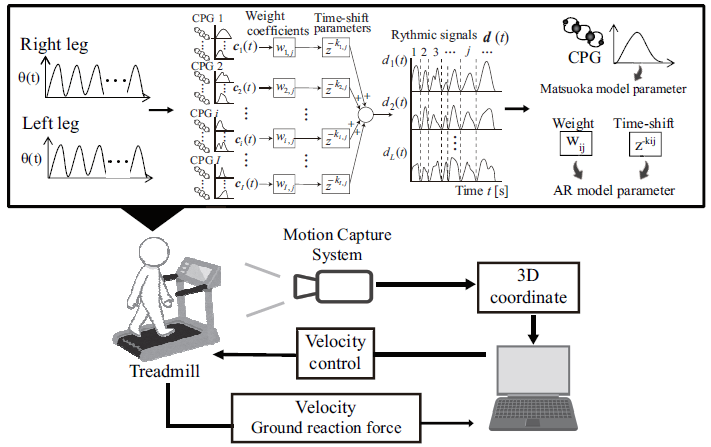
\includegraphics[width=\hsize]{fig/system.png}
\end{center}
\caption{Overview of the system}
 \label{system}
\end{figure}
\begin{figure}[H]
\begin{center}
 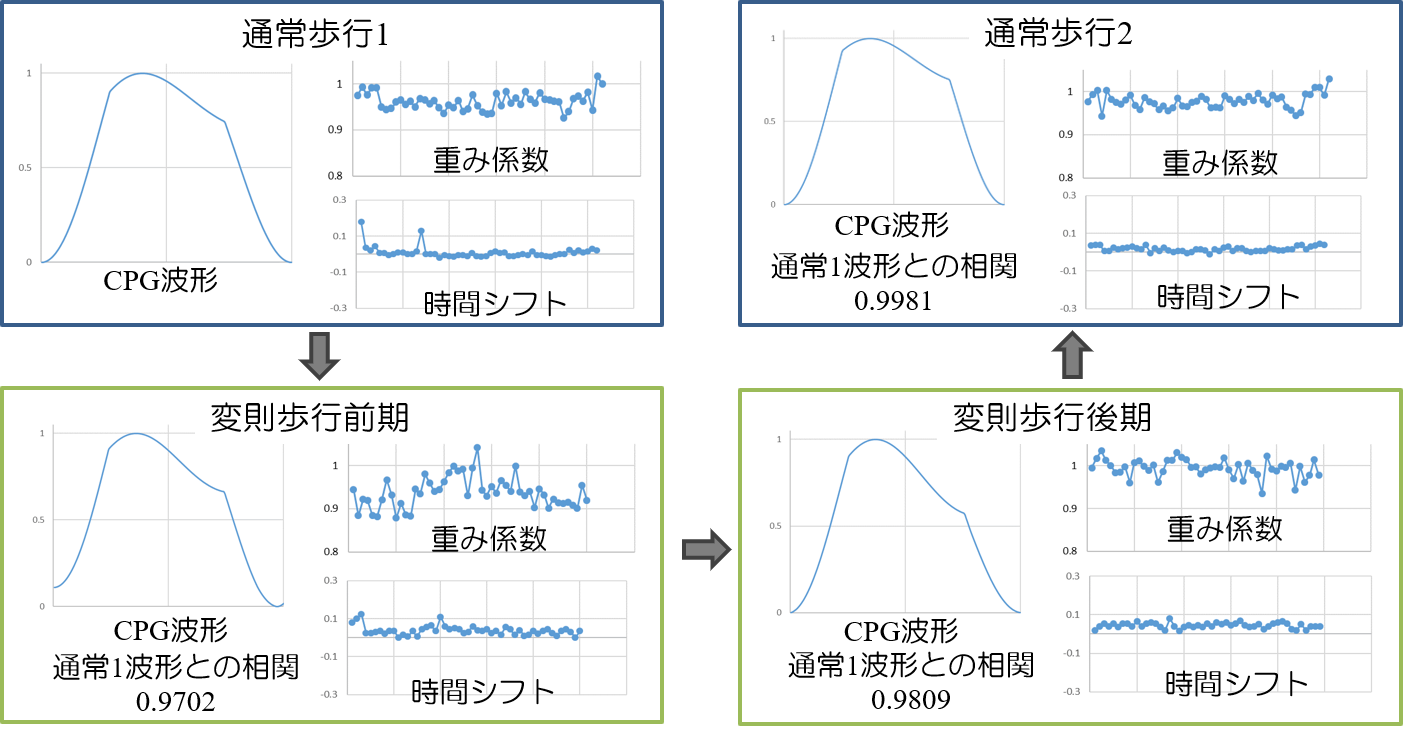
\includegraphics[width=\hsize]{fig/result.png}
\end{center}
\caption{Result of the analysis}
 \label{result}
\end{figure}
\begin{figure}[H]
\begin{center}
 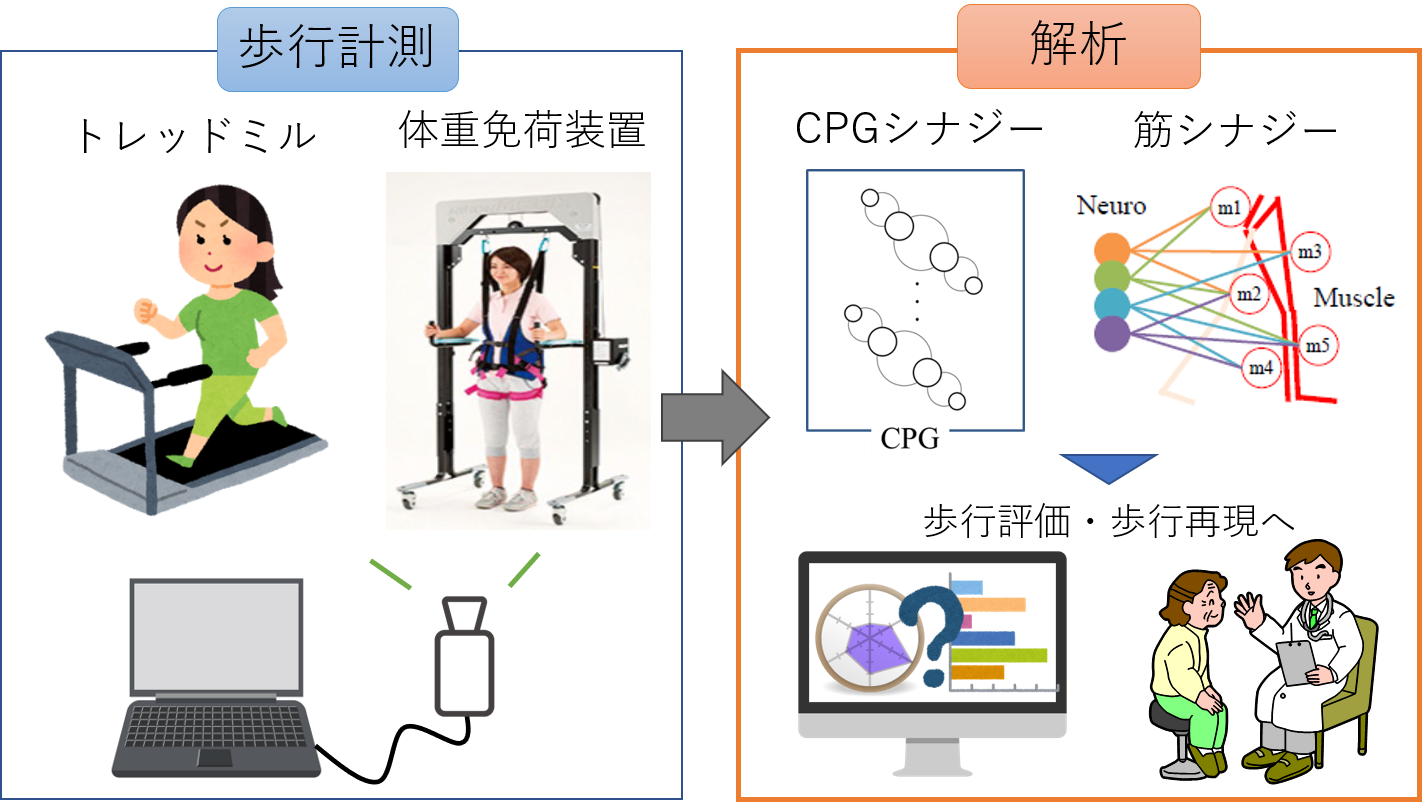
\includegraphics[width=\hsize]{fig/research.png}
\end{center}
\caption{Overview of the research}
 \label{research}
\end{figure}
%%%%%%%%%%%%%%%%%%%%%%%%%%%%%%%%


%% 著者:論文題目,誌名,\textbf{巻}-号,始ページ/終ページ(西暦)
%% 著者:書名,ページ,発行所名(発行西暦年)
\begin{thebibliography}{99}

%\bibitem{ziko}
%警察庁交通局 :  平成30年中の交通事故の発生状況
%https://www.npa.go.jp/news/release/2019/20190226001.html


\bibitem{elderly}
Cabinet Office,“Annual Report on the Aging Society: 2019”,p.2,2019.


\bibitem{neural1}
Reid K. F, Fielding R. A. ,“Skeletal muscle power: a critical determinant of
physical functioning in older adults”,Exerc Sport Sci Rev,Vol.40,No.1,pp.
4–12,2012.


\bibitem{neural2}
W.Marjorie H,Pei-Fang.Tang,“Balance control during walking in the older
adult: Research and its implications”,Physical Therapy,Vol.77,No.6,pp.
646–660,1997.


\bibitem{cpg}
S.Grillner,“Neurobiological bases of rhythmic motor acts in vertebrates”,Science,
Vol.228,No.4696,pp.143–149,1985.


\bibitem{human}
M.R.Dimitrijevic,T.Nomura,Y.Gerasimenko and M.M.Pinter,“ Evidence
for a spinal central pattern generator in humans”,Ann N.Y.Acad.Sci.
,Vol.860,pp.360–376,1998.


\bibitem{robot}
G.Taga,Y.Yamaguchi,H.Shimizu,“ Self-organized control of bipedal locomotion
by neural oscillators in unpredictable environment”,Biological Cybernetics,
Vol.65,No.3,pp.147–159,1991.


\bibitem{perkinson}
Y.Asai,T.Nomura,S.Sato,A.Tamaki,Y.Matsumoto,I.Mizukura and
K.Abe,“A coupled oscillator model of disordered interlimb coordination in patients
with Parkinson’s disease”,Biological Cybernetics,Vol.88,pp.152–162,
2003.


\bibitem{matsuoka}
K.Matsuoka,“ Sustained oscillations generated by mutually inhibiting neurons
with adptations” ,Biological Cybernetics,Vol.52,No.6,pp.367–376,1985.


\bibitem{kuramoto}
Y.Kuramoto,“Chemical Oscillations, Waves, and Turbulence”,Springer,1984.

\bibitem{infant}
Gauss Lee,Robert Lowe,Tom Ziemke,“Modelling Early Infant Walking: Testing
a Generic CPG Architecture on the NAO Humanoid”,IEEE International
Conference on Development and Learning,pp.1–6,2011.

\bibitem{impaired}
Naofumi Miura et al.,“Analyzing Compensation Strategy in Impaired Walking
Using a Humanoid Robot”,Transaction on control and mechanical sysytem,Vol.
1,No.1,pp.20–25,2012.


\bibitem{shima}
K.Shima et al.,“A CPG synergy model for evaluation of human finger tapping
movements”,2011 Annual International Conference of the IEEE Engineering in
Medicine and Biology Society,pp. 4443-4448,2011.


\bibitem{seo}
Akiho Seo,“Gait analysis method using CPG Synergy Model based nonlinear
oscillator”,Master Thesis,2020.


\end{thebibliography}


\end{document}



